% \documentclass[12pt,english]{article}
% \usepackage[utf8]{inputenc}
% \usepackage[left=1.5in,right=1.5in,top=1.5in,bottom=1.5in]{geometry}
% \usepackage{bm}
% \usepackage{amsmath}
% \usepackage{amssymb}
% \usepackage{indentfirst}
% \usepackage[hyperpageref]{backref} % back references biblio
% \usepackage{tocbibind}
% \usepackage[round,sort&compress]{natbib}
% \setcitestyle{aysep={}} 
% \usepackage{amsfonts}
% \usepackage{enumerate}
% \usepackage{babel}
% \usepackage{caption}
% \usepackage{supertabular}
% \usepackage{tabularx}
% \usepackage{float}
% \usepackage{dsfont}
% \usepackage{fancyvrb}
% \usepackage{verbatim}
% \usepackage[hyphens]{url}
% \usepackage{hyperref}
% \usepackage{enumitem}
% \usepackage{setspace}
% \usepackage{comment}
% \usepackage{subcaption}
% \usepackage{graphicx}
% \usepackage{tikz}
% \usepackage{gensymb}
% \usepackage{eurosym}
% \usepackage{textcomp}

% \usepackage{tabulary}
% \usepackage{tabularx}
% \usepackage{booktabs}
% \usepackage{fullpage}
% \usepackage{morefloats}
% % \usepackage[utf8]{inputenc}
% % \usepackage{bm}
% % \usepackage{indentfirst}
% % \usepackage{tocbibind}
% % \usepackage{enumerate}
% \usepackage{makecell}
% \usepackage{lscape}
% \usepackage{pdflscape}
% \usepackage{longtable}
% \usepackage{rotating}
% \usepackage{fancyhdr}
% \usepackage{tocloft}
% \usepackage{multibib}
% \usepackage{titletoc}
% \usepackage[export]{adjustbox}
% \usepackage[anythingbreaks]{breakurl} % for links
% %\usepackage[nomarkers,figuresonly]{endfloat} % Figures at the end
% \hypersetup{
%   colorlinks=true, % breaklinks=true,
%   urlcolor=purple,    % color of external links
%   linkcolor=blue,  % color of toc, list of figs etc.
%   citecolor=violet,   % color of links to bibliography
% }
% %\usepackage[section,below]{placeins} % Floats placed in the section they appear in.

% % Getting landscape page and page number/footer on bottom of page (instead of to the left)
% \fancypagestyle{mylandscape}{
% \fancyhf{} %Clears the header/footer
% \fancyfoot{% Footer
% \makebox[\textwidth][r]{% Right
%   \rlap{\hspace{1.5cm}% Push out of margin by \footskip
%     \smash{% Remove vertical height
%       \raisebox{13.6cm}{% Raise vertically
%         \rotatebox{90}{\thepage}}}}}}% Rotate counter-clockwise
% \renewcommand{\headrulewidth}{0pt}% No header rule
% \renewcommand{\footrulewidth}{0pt}% No footer rule
% }

% \fancypagestyle{page_left}{%
% 	\renewcommand{\headrulewidth}{0pt}
%   \fancyhf{}
%   \fancyfoot[OC]{%
%       \begin{tikzpicture}[remember picture,overlay]
%           \node[xshift=1cm] (number) at (current page.west) {\thepage};
%       \end{tikzpicture}
%   }%
% }
% \renewcommand{\thesubfigure}{\Alph{subfigure}}

% \newcites{App}{Appendix References}

% \captionsetup[table]{skip=-10pt}

% \title{International Attitudes Toward Global Policies \\ Addressing Climate Change and Inequality\thanks{Corresponding author: Fabre: CNRS, CIRED (fabre.adri1@gmail.com).
% Thomas Douenne: University of Amsterdam (t.r.g.r.douenne@uva.nl). Linus Mattauch: TU Berlin (linus.mattauch@tu-berlin.de). We are grateful for financial support from the University of Amsterdam and TU Berlin. We are grateful for financial support from the OECD, the French Ministry of Foreign Affairs, the French Conseil d’Analyse Economique and the Spanish Ministry for the Ecological Transition and Demographic Challenge. We also acknowledge support from the Grantham Foundation for the Protection of the Environment and the Economic and Social Research Council through the Centre for Climate Change Economics and Policy. We thank Antoine Dechezleprêtre, Tobias Kruse, Bluebery Planterose, Ana Sanchez Chico, and Stefanie Stantcheva for their invaluable inputs for the project. We thank Auriane Meilland for feedback. We thank Laura Schepp, Martín Fernández-Sánchez, Samuel Gervais, Samuel Haddad, and Guadalupe Manzo for assistance in the translation. The project %is approved by IRB at Harvard University (IRB21-0137), and 
% was preregistered in the Ooen Science Foundation registry (osf.io/fy6gd).}}
% %\author{OECD}
% \author{Adrien Fabre, Thomas Douenne, and Linus Mattauch}
% \date{\today}

% \begin{document}

% \maketitle

% \begin{small}
% \begin{abstract}

% \noindent \cite{dechezlepretre_fighting_2022-1} %Using new surveys on more than 40,000 respondents in twenty countries that account for 72\% of global CO$_\text{2}$ emissions, we study the understanding of and attitudes toward climate change and climate policies. We show that, across countries, support for climate policies hinges on three key perceptions centered around the effectiveness of the policies in reducing emissions (effectiveness concerns), their distributional impacts on lower-income households (inequality concerns), and their impact on the respondents' household (self-interest). We show experimentally that information  specifically addressing these key concerns can substantially increase the support for climate policies in many countries. Explaining how policies work and who can benefit from them is critical to foster policy support, whereas simply informing people about the impacts of climate change is not effective. Furthermore, we identify several socioeconomic and lifestyle factors -- most notably education, political leanings, and availability of public transportation -- that are significantly correlated with both policy views and overall reasoning and beliefs about climate policies. However, it is difficult to predict beliefs or policy views based on these characteristics only. 

% \end{abstract}

% \textbf{JEL codes:} P48, Q58, H23, Q54
% % Q54 Climate • Natural Disasters and Their Management • Global Warming
% % Q58 Government Policy (Q is Environmental econ)
% % D78 Positive Analysis of Policy Formulation and Implementation
% % H23 Externalities • Redistributive Effects • Environmental Taxes and Subsidies (H is public econ)
% % P48 Political Economy • Legal Institutions • Property Rights • Natural Resources • Energy • Environment • Regional Studies (P4 is Other economic systems)
% % H41 Public Goods
% % H54 Infrastructures • Other Public Investment and Capital Stock


% \textbf{Keywords:} Climate change, global policies, cap-and-trade, perceptions, survey, inequality, wealth tax.

% \end{small} 

% \clearpage
% % \startcontents
% % \printcontents{ }{1}{\section*{\contentsname}}
% % \clearpage
% \section{Introduction\label{sec:intro}}

% % \clearpage
% \renewcommand{\bibsection}{\section{\refname}}
% \bibliographystyle{naturemag}
% \bibliography{global_tax_attitudes}
% % \stopcontents

% \end{document}


\documentclass{nature}

% The following allows keeping figures within the text (otherwise nature.cls would ignore them)
\usepackage{graphicx}
\makeatletter
\let\saved@includegraphics\includegraphics
\AtBeginDocument{\let\includegraphics\saved@includegraphics}
\renewenvironment*{figure}{\@float{figure}}{\end@float}
\makeatother

\title{International Attitudes Toward Global Policies %\\ Addressing Climate Change and Inequality
} 

\author{Adrien Fabre$^{1,2}$, Thomas Douenne$^3$ and Linus Mattauch$^4$}


\begin{document}

% Nature guidelines (not NCC!)
% Sections can only be used in Articles.  Contributions should be organized in the sequence: title, text, methods, references, Supplementary Information line (if any), acknowledgements, interest declaration, corresponding author line, tables, figure legends.

% Spelling must be British English (Oxford English Dictionary)

%Each figure legend should begin with a brief title for the whole figure and continue with a short description of each panel and the symbols used. For contributions with methods sections, legends should not contain any details of methods, or exceed 100 words (fewer than 500 words in total for the whole paper). In contributions without methods sections, legends should be fewer than 300 words (800 words or fewer in total for the whole paper).

% Articles are restricted to 50 references,

% In addition, a cover letter needs to be written with the
% following:
% \begin{enumerate}
%  \item A 100 word or less summary indicating on scientific grounds
% why the paper should be considered for a wide-ranging journal like
% \textsl{Nature} instead of a more narrowly focussed journal.
%  \item A 100 word or less summary aimed at a non-scientific audience,
% written at the level of a national newspaper.  It may be used for
% \textsl{Nature}'s press release or other general publicity.
%  \item The cover letter should state clearly what is included as the
% submission, including number of figures, supporting manuscripts
% and any Supplementary Information (specifying number of items and
% format).
%  \item The cover letter should also state the number of
% words of text in the paper; the number of figures and parts of
% figures (for example, 4 figures, comprising 16 separate panels in
% total); a rough estimate of the desired final size of figures in
% terms of number of pages; and a full current postal address,
% telephone and fax numbers, and current e-mail address.
% \end{enumerate}

% See \textsl{Nature}'s website
% (\texttt{http://www.nature.com/nature/submit/gta/index.html}) for
% complete submission guidelines.

\maketitle

\begin{affiliations}
\item CNRS
\item CIRED
\item University of Amsterdam
\item TU Berlin
\end{affiliations}

\begin{abstract}
  \cite{dechezlepretre_fighting_2022-1}
\end{abstract}

% Intro

\begin{figure}
\caption{Points.}
\makebox[\textwidth][c]{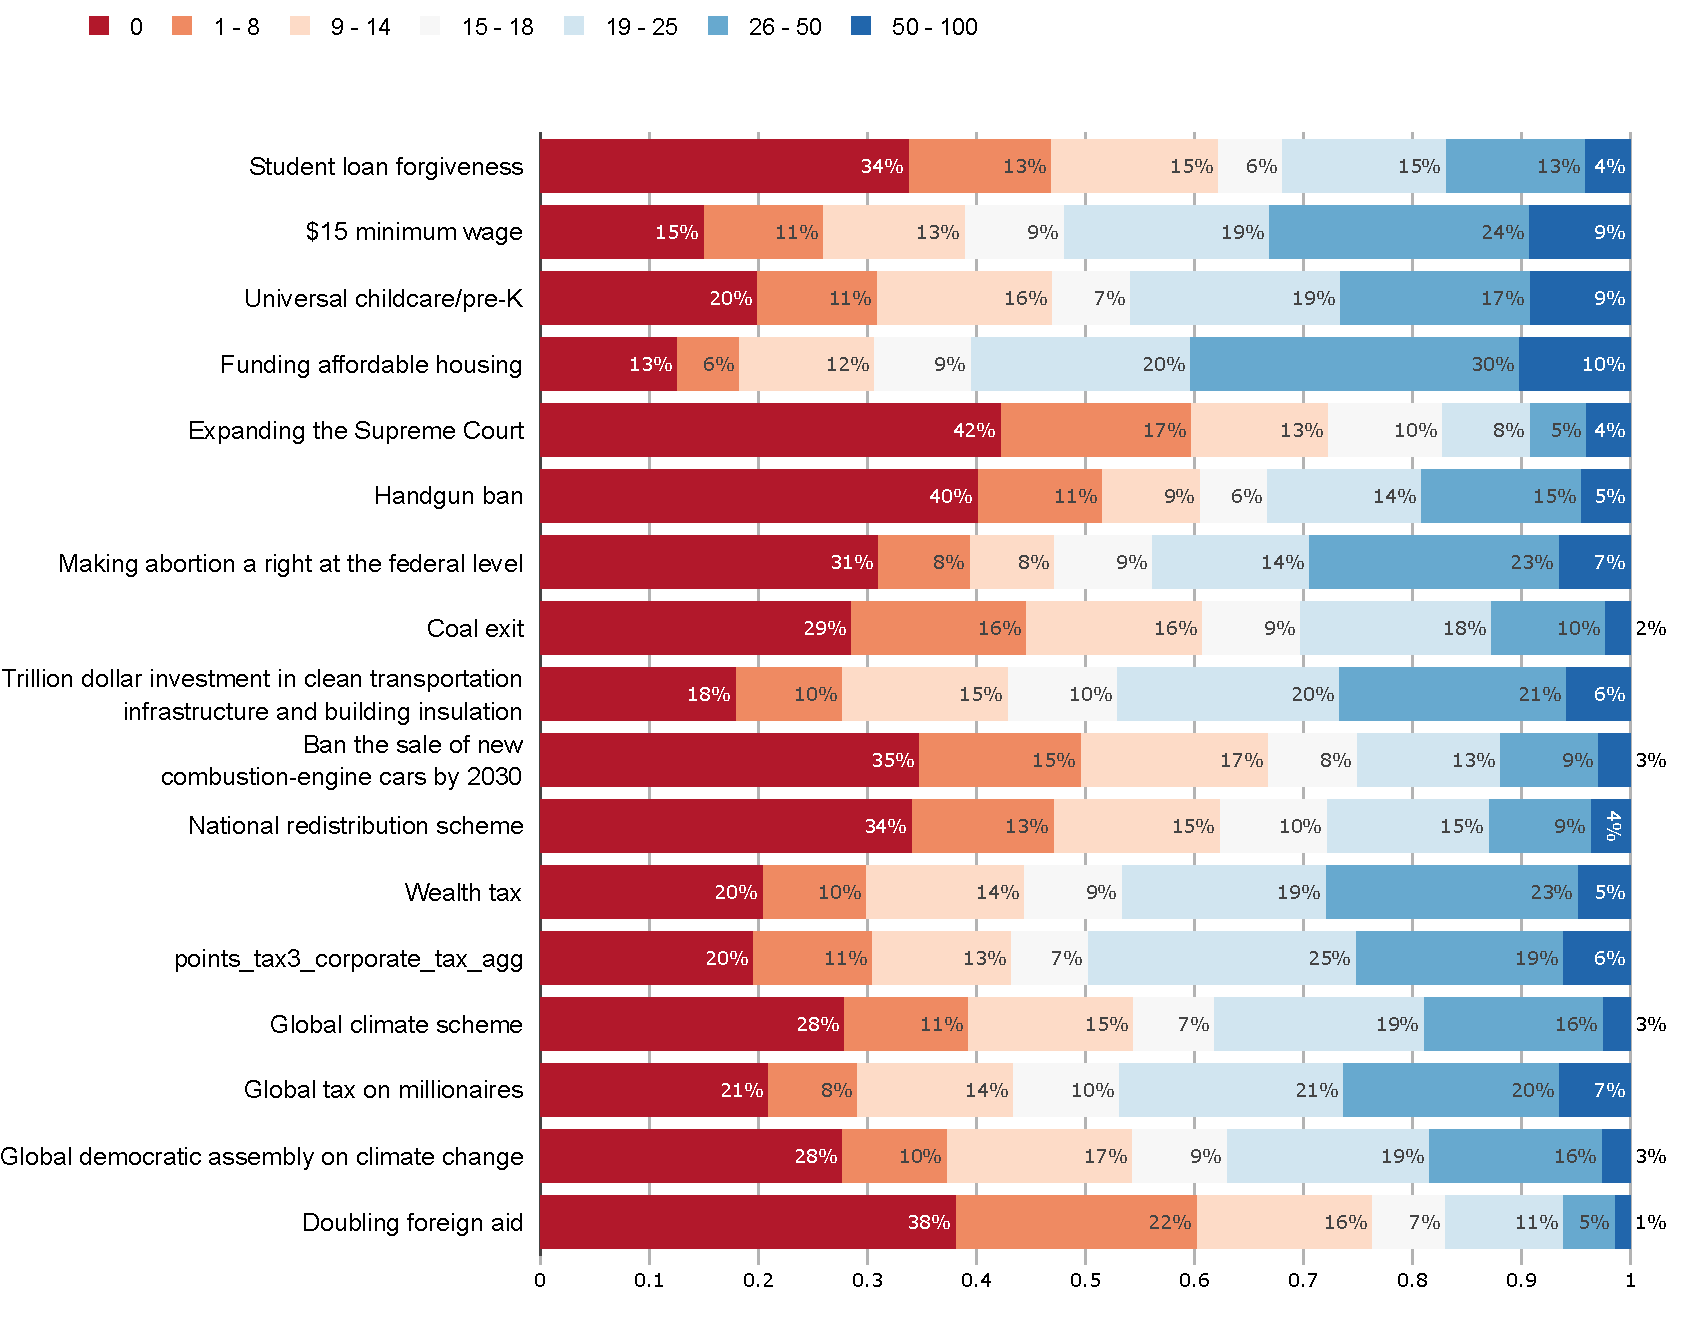
\includegraphics[width=.7\textwidth]{../figures/US1/points_us}}
\end{figure}

\section*{Results}

\section*{Discussion}


\begin{methods}
%Put methods in here.  If you are going to subsection it, use \subsection commands.  Methods section should be less than 800 words and if it is less than 200 words, it can be incorporated into the main text.

% \subsection{Method subsection.}

% Here is a description of a specific method used.  Note that the subsection heading ends with a full stop (period) and that the command is \verb|\subsection{}| not \verb|\subsection*{}|.

\end{methods}


\bibliographystyle{naturemag_noURL} % nature class works only with style naturemag or naturemag_noURL, and naturemag bugs if there are certain URLs (like .pdf). Also, nature class only works with \cite, not \citet or \citep.
\bibliography{global_tax_attitudes}


%% Here is the endmatter stuff: Supplementary Info, etc.
%% Use \item's to separate, default label is "Acknowledgements"
\begin{addendum} % 177 words
 \item We are grateful for financial support from the University of Amsterdam and TU Berlin. We are grateful for financial support from the OECD, the French Ministry of Foreign Affairs, the French Conseil d’Analyse Economique and the Spanish Ministry for the Ecological Transition and Demographic Challenge. We also acknowledge support from the Grantham Foundation for the Protection of the Environment and the Economic and Social Research Council through the Centre for Climate Change Economics and Policy. We thank Antoine Dechezleprêtre, Tobias Kruse, Bluebery Planterose, Ana Sanchez Chico, and Stefanie Stantcheva for their invaluable inputs for the project. We thank Auriane Meilland for feedback. We thank Laura Schepp, Martín Fernández-Sánchez, Samuel Gervais, Samuel Haddad, and Guadalupe Manzo for assistance in the translation. 
 \item[Registration] The project %is approved by IRB at Harvard University (IRB21-0137), and 
 was preregistered in the Ooen Science Foundation registry (osf.io/fy6gd).
 \item[Competing Interests] The authors declare that they have no
competing interests.
\item[JEL codes] P48, Q58, H23, Q54.
\item[Keywords] Climate change, global policies, cap-and-trade, perceptions, survey, inequality, wealth tax.
 \item[Correspondence] Correspondence and requests for materials
should be addressed to Adrien Fabre~(email: fabre.adri1@gmail.com).
\end{addendum}

%%
%% TABLES
%%
%% If there are any tables, put them here.
%%

% \begin{table}
% \centering
% \caption{This is a table with scientific results.}
% \medskip
% \begin{tabular}{ccccc}
% \hline
% 1 & 2 & 3 & 4 & 5\\
% \hline
% aaa & bbb & ccc & ddd & eee\\
% aaaa & bbbb & cccc & dddd & eeee\\
% aaaaa & bbbbb & ccccc & ddddd & eeeee\\
% aaaaaa & bbbbbb & cccccc & dddddd & eeeeee\\
% 1.000 & 2.000 & 3.000 & 4.000 & 5.000\\
% \hline
% \end{tabular}
% \end{table}

\end{document}
